\documentclass[11pt,a4paper]{article}
\usepackage[utf8]{inputenc}
\usepackage[spanish]{babel}	%Idioma
\usepackage{amsmath}
\usepackage{amsfonts}
\usepackage{amssymb}
\usepackage{graphicx} 	%Añadir imágenes
\usepackage{geometry}	%Ajustar márgenes
\usepackage[export]{adjustbox}[2011/08/13]
\usepackage{float}
\restylefloat{table}
\usepackage[hidelinks]{hyperref}
\usepackage{titling}
\graphicspath{{/home/nazaret/Escritorio/LaTEX}}
\usepackage{subcaption} 
\usepackage{multirow}
\usepackage{caption}
\usepackage{multicol}
\usepackage[shortlabels]{enumitem}
\usepackage{array}
\selectlanguage{spanish}

%Opciones de encabezado y pie de página:
\usepackage{fancyhdr}
\pagestyle{fancy}
\lhead{Nazaret Román Guerrero}
\rhead{Procesamiento Digital de Señales}
\lfoot{Grado en Ingeniería Informática}
\cfoot{}
\rfoot{\thepage}
\renewcommand{\headrulewidth}{0.4pt}
\renewcommand{\footrulewidth}{0.4pt}

%Opciones de fuente:
\usepackage[utf8]{inputenc}
\usepackage[default]{sourcesanspro}
\usepackage{sourcecodepro}
\usepackage[T1]{fontenc}

\setlength{\parindent}{15pt}
\setlength{\headheight}{15pt}
\setlength{\voffset}{10mm}

% Custom colors
\usepackage{color}
\definecolor{deepblue}{rgb}{0,0,0.5}
\definecolor{deepred}{rgb}{0.6,0,0}
\definecolor{deepgreen}{rgb}{0,0.5,0}

\usepackage{listings}
\usepackage{color}
\usepackage{graphicx}

\definecolor{dkgreen}{rgb}{0,0.6,0}
\definecolor{gray}{rgb}{0.5,0.5,0.5}
\definecolor{mauve}{rgb}{0.58,0,0.82}

\lstset{frame=tb,
  language=Matlab,
  aboveskip=3mm,
  belowskip=3mm,
  showstringspaces=false,
  columns=flexible,
  basicstyle={\small\ttfamily},
  numbers=left,
  numberstyle=\tiny\color{gray},
  keywordstyle=\color{blue},
  commentstyle=\color{dkgreen},
  stringstyle=\color{mauve},
  breaklines=true,
  breakatwhitespace=true,
  tabsize=4
}

\begin{document}
\begin{titlepage}

\begin{minipage}{\textwidth}

\centering

\includegraphics[width=0.55\textwidth]{img/logo.png}\\

\textsc{\Large Procesamiento Digital de Señales\\[0.2cm]}
\textsc{GRADO EN INGENIERÍA INFORMÁTICA}\\[1cm]

{\Huge\bfseries Práctica 5\\}
\noindent\rule[-1ex]{\textwidth}{3pt}\\[3.5ex]
{\large\bfseries Diseño de filtros digitales FIR}
\end{minipage}

\vspace{1.5cm}
\begin{minipage}{\textwidth}
\centering

\textbf{Autora}\\ {Nazaret Román Guerrero}\\[2.5ex]

\includegraphics[width=0.3\textwidth]{img/etsiit.jpeg}\\[0.1cm]
\vspace{1cm}
\textsc{Escuela Técnica Superior de Ingenierías Informática y de Telecomunicación}\\
\vspace{1cm}
\textsc{Curso 2018-2019}
\end{minipage}
\end{titlepage}

\pagenumbering{gobble}
\pagenumbering{arabic}
\tableofcontents
\thispagestyle{empty}

\newpage

Para esta práctica se ha utilizado un intérprete online de Matlab. El intérprete es el mismo que en las demás prácticas: \color{blue} \url{https://octave-online.net/}\color{black}.

\section{Filtro FIR con ventana rectangular}
 Para este ejercicio, el código se puede leer en \color{deepred}\nameref{code1}\color{black}. Además, está incluido con el nombre \texttt{fir\_ventana.m}.\\
 
A pesar de que el código está explicado, lo voy a desarrollar un poco más. Lo primero es establecer las especificaciones que se indican en la práctica, indicando el número de muestras del filtro (\texttt{M}) y las frecuencias de muestreo y de corte (\texttt{Fs} y \texttt{Fc} respectivamente). A partir de estas frecuencias calculamos wc. Ya que no sabía por qué \texttt{wc} siempre era 0.5 en las transparencias de clase, busqué en Internet y vi que provenía de una operación simple entre las frecuencias de corte y de muestreo, como se puede ver en el código.\\

Una vez hecho esto, creamos una ventana rectangular mediante la función \texttt{rectwin(M)}, que crea una ventana con el número de muestras del filtro. Debemos ajustarla con la función \texttt{reshape} porque de lo contrario Matlab no puede sacar la gráfica, ya que no coincide la estructura de datos que requiere para pintarla.\\

Generamos el impulso ideal y calculamos la salida de $H_d$ con la ventana que habíamos creado antes.\\

Después solamente tenemos que sacar la gráfica, que nos muestra lo siguiente:

\begin{figure}[H]
	\centering
	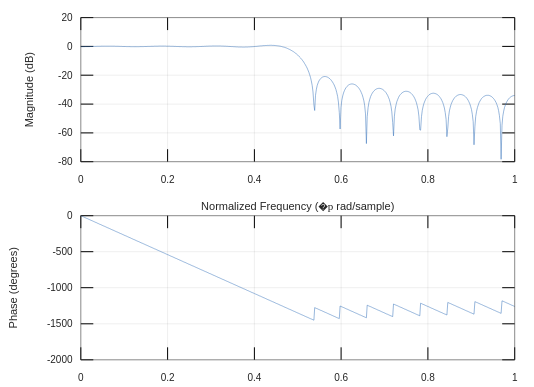
\includegraphics[scale=0.5]{img/1.png}
\end{figure}
 
Como podemos ver, es un filtro paso baja puesto que la respuesta en frecuencia está dejando pasar las frecuencias bajas pero no las altas.

\begin{itemize}
	\item \textbf{¿Qué modificaciones introduciría en el diseño del filtro para conseguir una atenuación de -50 dB para el primer lóbulo de la banda de atenuación con la mayor pendiente posible en la banda de transición?}
\end{itemize}

Para que se produzca una atenuación en los lóbulos de la banda es necesario que disminuya el número de coeficientes del filtro, de forma que la caída se hace menos abrupta pero más profunda es decir, la pendiente es menor pero la atenuación es mayor. Si queremos que llegue a una atenuación de -50 dB utilizamos 15 coeficientes para el filtro.\\

Para ello solo debemos cambiar una línea en el código:

\begin{lstlisting}[frame=single]
% Se definen los parametros
% Numero de coeficientes del filtro
M=15
\end{lstlisting}

La respuesta en frecuencia con \texttt{M=15} es la siguiente:

\begin{figure}[H]
	\centering
	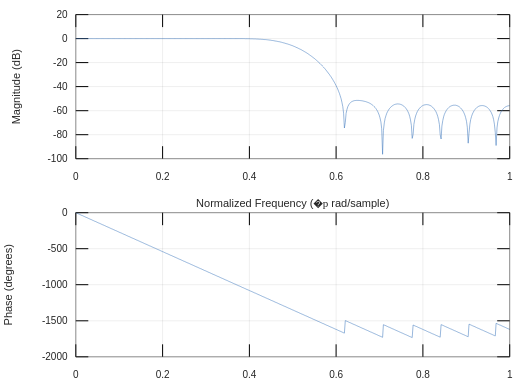
\includegraphics[scale=0.5]{img/2.png}
\end{figure}

Como podemos ver, la pendiente del primer lóbulo es menor que con más coeficientes, pero sin embargo ha superado los -50 dB de atenuación que ibamos buscando.

\newpage

\section{Filtro FIR con \texttt{fir1}}

En este caso vamos a utilizar la función \texttt{fir1}. Vamos a hacer dos cosas: primero, comparar la respuesta en frecuencia del filtro con distintas \texttt{M}, y después con una \texttt{M} fija pero con distintos tipos de ventanas.

\subsection{Comparativa de M}

Vamos a comenzar con la comparativa de las distintas \texttt{M}. En la última columna de la tabla se incluye un enlace a cada sección del anexo con el código correspondiente en cada caso.

\begin{table}[H]
\begin{tabular}{|c|c|c|c|c|}
\hline
M  & Anchura & Atenuación & Respuesta en frecuencia & Sección con el código \\ \hline
15 & \textasciitilde{} Hz            & \textasciitilde{}42 dB                       & 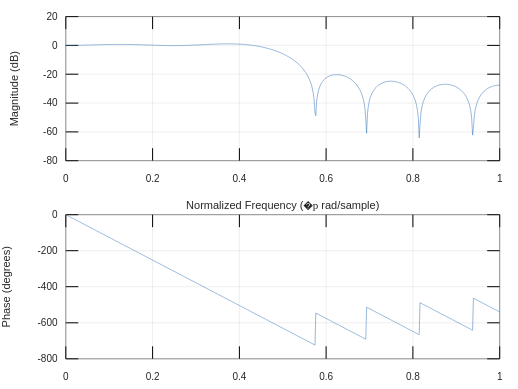
\includegraphics[scale=0.3]{img/3.png} &  \color{deepred}\nameref{code2}\color{black} \\ \hline
31 & \textasciitilde{} Hz            & \textasciitilde{}60 dB                       & 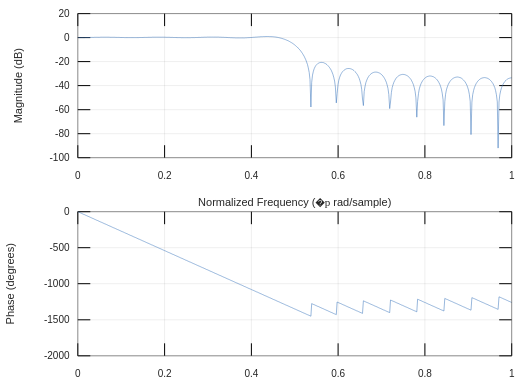
\includegraphics[scale=0.3]{img/4.png} & \color{deepred}\nameref{code3}\color{black} \\ \hline
63 & \textasciitilde{} Hz            & \textasciitilde{}40 dB                       & 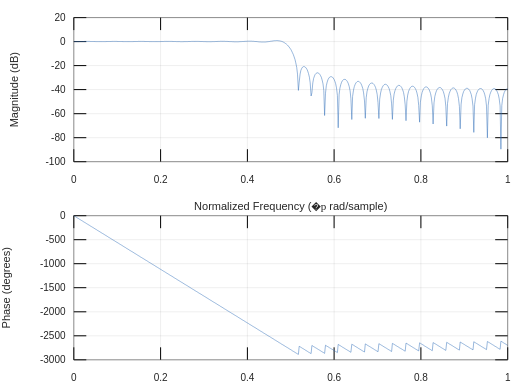
\includegraphics[scale=0.3]{img/5.png} & \color{deepred}\nameref{code4}\color{black} \\ \hline
\end{tabular}
\caption{Tabla comparativa de M}
\end{table}

Como podemos ver en las imágenes, cuantos más coeficientes tiene el filtro, mayor es la pendiente del primer lóbulo, lo cual lo hace más realista. Cuando \texttt{M} tiende a infinito la respuesta en frecuencia tiende a la respuesta ideal, por eso cuanto más coeficientes, más precisa es la salida.

\subsection{Comparativa de enventanado}

Ahora vamos a llevar a cabo la comparativa entre los distintos tipos de ventanas utilizando un número fijo de coeficientes, que se corresponde con \texttt{M=31}. Al igual que en la tabla anterior, cada código se puede ver pulsando el enlace de la última columna a la tabla.

\begin{table}[H]
\begin{tabular}{|c|c|c|c|c|}
\hline
Ventana  & Anchura & Atenuación & Respuesta en frecuencia & Sección con el código \\ \hline
Rectangular & \textasciitilde{} Hz            & \textasciitilde{}60 dB                       & 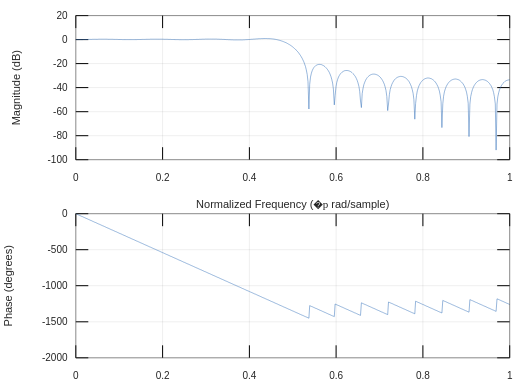
\includegraphics[scale=0.25]{img/6.png} &  \color{deepred}\nameref{code5}\color{black} \\ \hline
Bartlett & \textasciitilde{} Hz            & \textasciitilde{}25 dB                       & 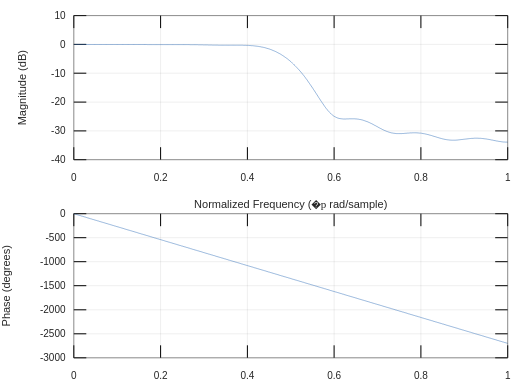
\includegraphics[scale=0.25]{img/7.png} & \color{deepred}\nameref{code6}\color{black} \\ \hline
Hamming & \textasciitilde{} Hz            & \textasciitilde{}100 dB                       & 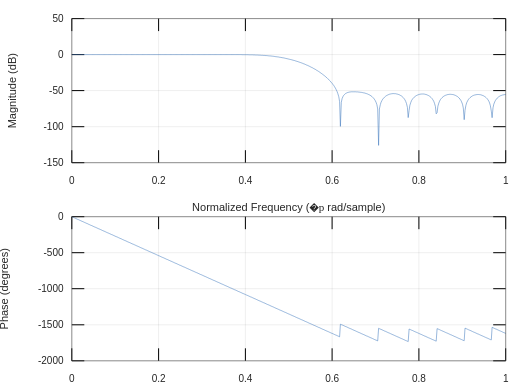
\includegraphics[scale=0.25]{img/8.png} & \color{deepred}\nameref{code7}\color{black} \\ \hline
\end{tabular}
\caption{Tabla comparativa de ventanas}
\end{table}

La diferencia entre los tres tipos de ventanas es evidente. Como podemos ver, la ventana Hamming es la que tiene una mayor atenuación, llegando hasta -100 dB en el primer lóbulo. Por el contrario, la ventana Bartlett solo alcanza los 25 dB; además, con esta última ventana, no se ven lóbulos propiamente dichos, se ven pequeñas ondas a lo largo de la gráfica con la respuesta en frecuencia.

\newpage

\subsection{Filtro con \texttt{fir2}}

El código de este apartado está incluido con el nombre de \texttt{fir2.m}; también se puede ver en \color{deepred}\nameref{code8}\color{black}. Ya que para hacer este ejercicio he dependido de la documentación de Matlab, voy a explicar un poco lo que he hecho.

Según la documentación de la función \texttt{fir2}, en el ejemplo se utilizan 34 coeficientes, y como no estaba muy segura de por qué, probé con el valor de \texttt{M} que había estado utilizando en los ejercicios anteriores, con \texttt{M=31}; no obstante, el filtro no tenía casi atenuación y no sabía por qué, así que dejé los coeficientes del ejemplo.\\

Para utilizar la función, se requiere un vector  con la frecuencia de las bandas. Como la frecuencia de corte es 4000 Hz, imponemos esta frecuencia como la frecuencia de las bandas. Para establecer 4 kHz como la frecuencia de corte, debemos utilizarla dos veces, y establecer en el vector de amplitudes que es el punto donde se empiezan a tomar las frecuencias para hacer el filtro paso alta.\\

En el vector de amplitud se establece la magnitud de las frecuencias; es decir, aquellas que estén a 0 no serán tenidas en cuenta, aquellas que estén a 1 se tendrán en cuenta. En el caso de la frecuencia de corte hay que establecer que es la frecuencia de corte imponiendo que ésta se toma y a la vez no se toma como parte del filtro: debe tener un valor 0 asignado y también un valor 1. Por este motivo es por el que está duplicada la frecuencia en el vector de frecuencias de las bandas.\\

Finalmente se calcula la respuesta en frecuencia del filtro usando \texttt{fir2}. La salida es la siguiente:

\begin{figure}[H]
	\centering
	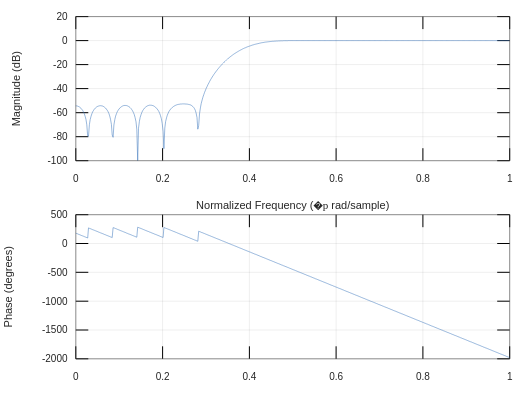
\includegraphics[scale=0.5]{img/9.png}
\end{figure}

Como podemos ver, tenemos un filtro paso alta con frecuencia de corte en 0.4 (las frecuencias están normalizadas en la gráfica).

\newpage

\section{Anexo: Códigos fuente}

\subsection{Filtro FIR con ventana rectangular}
\label{code1}

\begin{lstlisting}[frame=single]
% Se definen los parametros
% Numero de coeficientes del filtro
M=31

% Frecuencias de muestreo y de corte
Fs=8000
Fc=2000

% Calculamos la frecuencia de corte que usaremos
wc=Fc/(Fs/2)

% Parametros del filtro
N=(M-1)/2
n=0:1:M-1

% Ventana rectangular. Se redimensiona para pintarlo en la grafica
window = rectwin(M)
window = reshape(window, [1 31])

% Generamos el impulso
hd=wc*sinc((n-N)*wc)

% Calculamos la salida del filtro y truncamos con la ventana
h=window.*hd

% Pintamos las graficas
freqz(h,1)
\end{lstlisting}

\subsection{Filtro FIR con fir1 y M=15}
\label{code2}

Incluido bajo el nombre de \texttt{filtro\_fir\_15.m}.

\begin{lstlisting}[frame=single]
% Coeficientes del filtro
M=15

% Frecuencias de muestreo y corte
Fs=8000
Fc=2000
wc=Fc/(Fs/2)

h = fir1(M-1, wc, rectwin(M))

freqz(h,1)
\end{lstlisting}

\subsection{Filtro FIR con fir1 y M=31}
\label{code3}

Incluido con el nombre de \texttt{filtro\_fir\_31.m}.

\begin{lstlisting}[frame=single]
% Coeficientes del filtro
M=31

% Frecuencias de muestreo y corte
Fs=8000
Fc=2000
wc=Fc/(Fs/2)

h = fir1(M-1, wc, rectwin(M))

freqz(h,1)
\end{lstlisting}

\subsection{Filtro FIR con fir1 y M=63}
\label{code4}

Código incluido como \texttt{filtro\_fir\_63.m}.

\begin{lstlisting}[frame=single]
% Coeficientes del filtro
M=63

% Frecuencias de muestreo y corte
Fs=8000
Fc=2000
wc=Fc/(Fs/2)

h = fir1(M-1, wc, rectwin(M))

freqz(h,1)
\end{lstlisting}

\subsection{Filtro FIR (rectangular)}
\label{code5}

Incluido como \texttt{fir\_rectangular.m}.

\begin{lstlisting}[frame=single]
% Coeficientes del filtro
M=31

% Frecuencias de muestreo y corte
Fs=8000
Fc=2000
wc=Fc/(Fs/2)

h = fir1(M-1, wc, rectwin(M))

freqz(h,1)
\end{lstlisting}

\subsection{Filtro FIR (bartlett)}
\label{code6}

Código incluido como \texttt{fir\_bartlett.m}.

\begin{lstlisting}[frame=single]
% Coeficientes del filtro
M=31

% Frecuencias de muestreo y corte
Fs=8000
Fc=2000
wc=Fc/(Fs/2)

h = fir1(M-1, wc, bartlett(M))

freqz(h,1)
\end{lstlisting}

\subsection{Filtro FIR (hamming)}
\label{code7}

Incluido en el \texttt{.zip} como \texttt{fir\_hamming.m}.

\begin{lstlisting}[frame=single]
% Coeficientes del filtro
M=31

% Frecuencias de muestreo y corte
Fs=8000
Fc=2000
wc=Fc/(Fs/2)

h = fir1(M-1, wc, hamming(M))

freqz(h,1)
\end{lstlisting}

\subsection{Filtro FIR con fir2}
\label{code8}

\begin{lstlisting}[frame=single]
% Coeficientes del filtro
M=34

% Debemos definir las bandas de frecuencia ya que fir2 necesita un vector con ellas

% Como la frecuencia de corte es 4kHz y el vector debe empezar en 0 y acabar en 1, las bandas que se van a tocar son las de 0.4
f=[0 0.4 0.4 1]


% Se define la amplitud de cada banda de frecuencia del vector f
amplitud = [0 0 1 1]

% Se devuelven M+1 coeficientes
h = fir2(M, f, amplitud)

freqz(h,1)

\end{lstlisting}

\end{document}